\section{Prediction tasks}
In this section, we grab the phenomenon surrounding around community process of Stack Overflow question-answering. We demonstrate prediction of value of a question to the community and to the questioner in two subtasks: Predicting the long-term value of a question and predicting whether the has been sufficiently answered or not.
\subsection{Predicting long-lasting value}

\begin{figure}[!t]
    \centering
    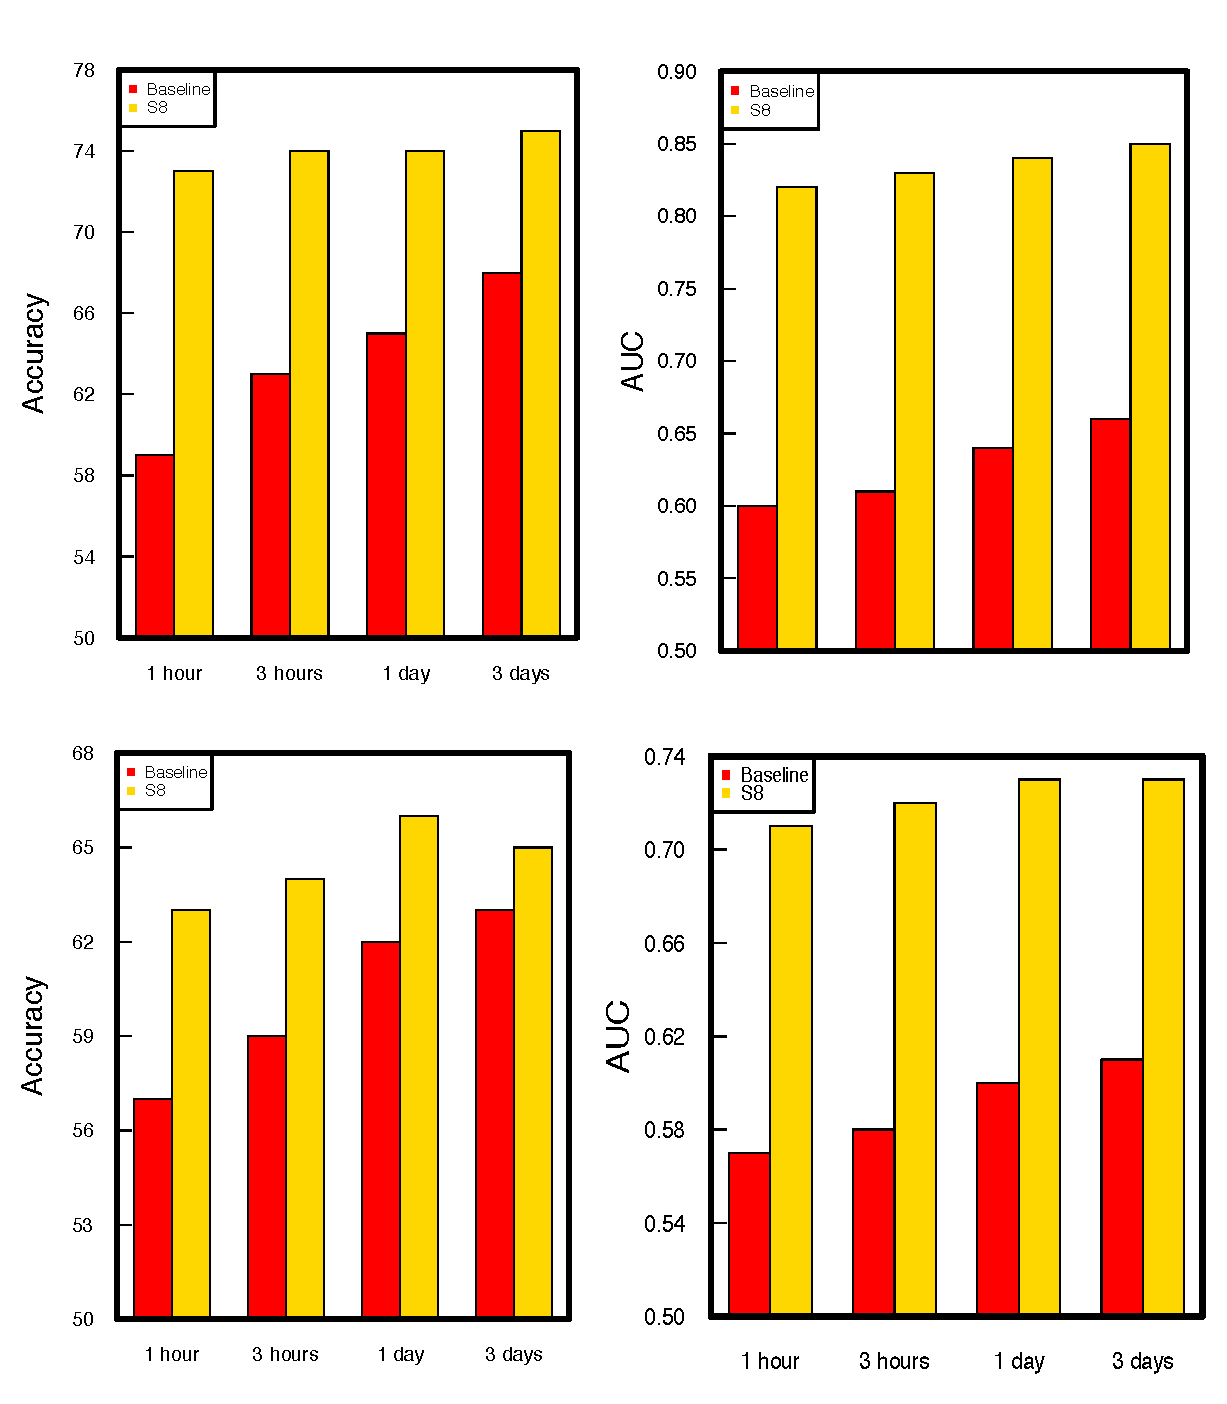
\includegraphics[width=0.7\columnwidth]{img/task1.pdf}
    \caption{Results of pageview prediction. Notice strong absolute and also relative performance of our method. (left) Accuracy, (right) Area under ROC curve. Top row is for quartile division of page view, bottom row is for half division of page view.}
    \label{fig:task1}
\end{figure}


\begin{table*}[]
	\centering
	\small
	\caption{Features used for learning}
	\label{tab:pred}
\begin{tabular}{|l|l|}
\hline
Questioner features (SA)               & \begin{tabular}[c]{@{}l@{}}questioner reputation, \# of questioner’s questions and answers, questioner’s, \\ percentage of accepted answers on their previous questions.\end{tabular}                                                                                                                                                                                                                            \\ \hline
Activity and Q/A quality measures (SB) & \begin{tabular}[c]{@{}l@{}}\# of favorites, \# of page views, \# positive and negative votes on question, \\ \# of answers, maximum answerer reputation, highest answer score, \\ reputation of answerer who wrote highest scoring answer.\end{tabular}                                                                                                                                                          \\ \hline
Community process features (SC)        & \begin{tabular}[c]{@{}l@{}}answerer reputation, median answerer reputation, fraction of sum of answerer \\ reputations contributed by max answerer  reputation, sum of answerer reputations, \\ length of answer by highest-reputation answerer, \# of comments on answer by \\ highest-reputation answerer, length of highest-scoring answer, \\ \# of comments on highest-scoring answer.\end{tabular}         \\ \hline
Temporal process features (SD)         & \begin{tabular}[c]{@{}l@{}}Average time between answers, median time between answers, \\ minimum time between answers, time-rank of highest-scoring answer, \\ wall-clock time elapsed between question creation and highest-scoring answer, \\ time-rank of answer by highest reputation answerer, wall-clock time elapsed between \\ question creation and answer by highest-reputation answerer.\end{tabular} \\ \hline
\end{tabular}
\end{table*}


\begin{table}[]
	\centering
	\small
	\caption{Feature coefficients for prediction task 1}
	\label{tab:8features}
	\resizebox{\columnwidth}{!}{%
\begin{tabular}{l|c}
Feature                                                   & Coefficient \\ \hline
Number of answers +0.61                                   & + 0.09      \\
Sum of answer scores +0.47                                & + 4.72      \\
\# of questioner’s questions (log scale) -0.46            & - 0.21      \\
Length of highest-scoring answer +0.38                    & + 0.08      \\
Questioner’s reputation (log scale) +0.31                 & + 0.05      \\
Time for highest-scoring answer to arrive +0.22           & + 0.34      \\
\# comments on highest-scoring answer +0.19               & + 0.23      \\
\# comments on highest-reputation answerer’s answer +0.17 & + 0.07      \\ \hline
\end{tabular}}
\end{table}


The community value of a question can be reflected in the long-term impact of a question. While, multiple features like “favourite count” , “Page Views”, “Up Votes” and “Down Votes reflect the impact of the question, page view has chosen to be a balanced feature as it is the reflector of a question’s value. Unlike up votes, down votes and favourite count; page view has a significantly large value. However, the number of page views can pose to be noisy and need pre-processing before prediction tasks. 
The features that have been found out from the previous sections include: questioners’ factors, activity and Q/A factors, community factors, and temporal factors as shown in Table \ref{tab:pred}.


\begin{figure}[!t]
    \centering
    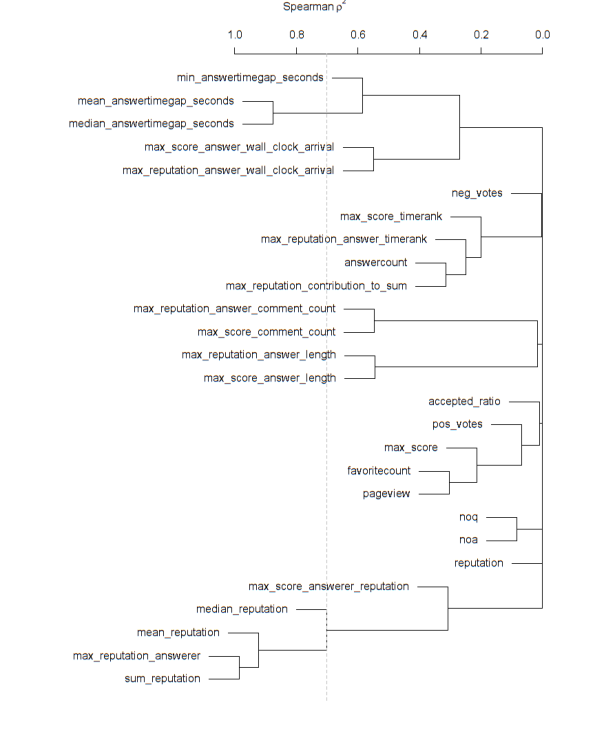
\includegraphics[width=\columnwidth]{img/Spearman.pdf}
    \caption{Hierarchical clustering of variables according to Spearman’s correlation}
    \label{fig:spearman}
\end{figure}


\textbf{Experiment Setup} To perform this prediction, we split the page view value into high and low. In the first case, this division is done by the mean, and data is split into half across the mean. In the second case, page view is split into 4 quadrants, taking the top most and the bottom most quartiles as high and low respectively. Quartile split provides reinforcement to the learnings and important features found in the case where page views are split by half. We reduced the questions with pageviews more than 5 million, to remove outliers and for generalizability of results.

Providing adequate time for a questions’ pageview value to mature itself is vital for the experiment. All the questions posted within the same month, 1 year before the last update of the stack-overflow data dump (31st December 2011) have been considered for the study, i.e. we considered questions with creation date between 1st December 2010 and 31st December 2010.  Most features required to predict the long-term value of a question arrive within a specified time of when question was posted. To further analyse this, we have predicted the model taking all features in 1, 3, 24 and 72 hour time-frames.

From the initial set of 27 features, we have performed correlation analysis, redundancy analysis and backward feature selection to obtain a core set of 8 features that sufficiently predict the long-term value of a question. In Fig \ref{fig:spearman}, we found that maximum reputation answer, sum of reputation, mean reputation were highly correlated to median reputation. Median reputation has been considered to reduce the total number of branches in the dendrogram. Redundancy analysis results concluded that the minimum time-gap between answers was a redundant feature. From the remaining set of 23 features, we performed downward feature selection to find a core set of 8 features as given in Table~\ref{tab:8features}. The coefficients in the figure reflect the effect of the features in predicting the high and low values of quartile page views for questions with features computed up to 3 days.

The results conclude that number of answers, sum of answer scores, number of questioner’s questions, length of highest scoring answer, time for highest scoring answer to arrive, number of comments on highest scoring answer, and comments on the highest reputation answerer’s answer impact the long-lasting value of a question. 
A comparison has been made with respect to baseline features. The model built with baseline features considers two features, sum of upvotes – sum of downvotes of a question, and the number of favourites of the question. 
In Fig~\ref{fig:task1} the AUC value increases less than 2 AUC units from one hour to three-hour time-frame. Similar is the case for accuracy value. The results demonstrate that most of the information required to predict the value of the question is obtained in 1 hour of the creation time of the question. 

\subsection{Predicting whether the question has been sufficiently answered}
Bounties are questioner’s way of expressing whether their questions have been sufficiently answered or not. Users with reputation lower than the minimum value required by Stack Exchange for posting bounties, do not experience the freedom to stress the value of their question.
For each question with bounty, we observe ‘k’ number of answers after which bounty was offered; and take a random sample of questions for which an answer was accepted after ‘k’ number of answers. To make the experiment fair, only the non-bounty questions, with questioner’s reputations lesser than the minimum required amount (75 reputation points) have been considered. 
The set of features Sa, Sb, Sc, Sd have been considered, taking Sa as the baseline. Since, the value of ‘k’ is constant for the experiment, answerers features remain constant per value of k. Addition of answerers features have been done in the original set of features Sa, Sb, Sc, Sd to update to Sa`, Sb`, Sc`, Sd` as shown in the table.

\begin{itemize}
	\item Sa` = Sa
	\item Sb` = Sb
	\item Sc` = Sa + (Sum of Upvotes + Sum of Down-Votes + Sum Answerers’ Reputation for each answer) 
	\item Sd` = Sd + (Time gap between answers)
\end{itemize}


\begin{table}[]
	\centering
	\small
	\caption{Number of questions after which bounty is offered}
	\label{tab:kvalues}
\begin{tabular}{|r|r|}
\hline
\multicolumn{1}{|c|}{k} & \multicolumn{1}{c|}{\#records} \\ \hline
1                       & 7810                           \\ \hline
2                       & 3208                           \\ \hline
3                       & 1406                           \\ \hline
4                       & 640                            \\ \hline
5                       & 276                            \\ \hline
6                       & 138                            \\ \hline
7                       & 110                            \\ \hline
8                       & 44                             \\ \hline
9                       & 34                             \\ \hline
10                      & 22                             \\ \hline
11                      & 12                             \\ \hline
12                      & 10                             \\ \hline
\end{tabular}
\end{table}


\begin{figure}[!t]
    \centering
    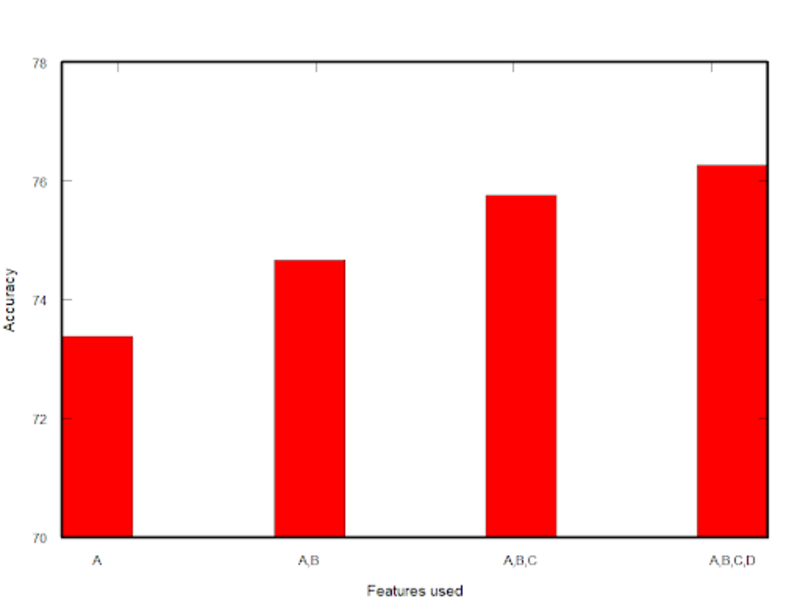
\includegraphics[width=0.7\columnwidth]{img/Fig10_left.pdf}
    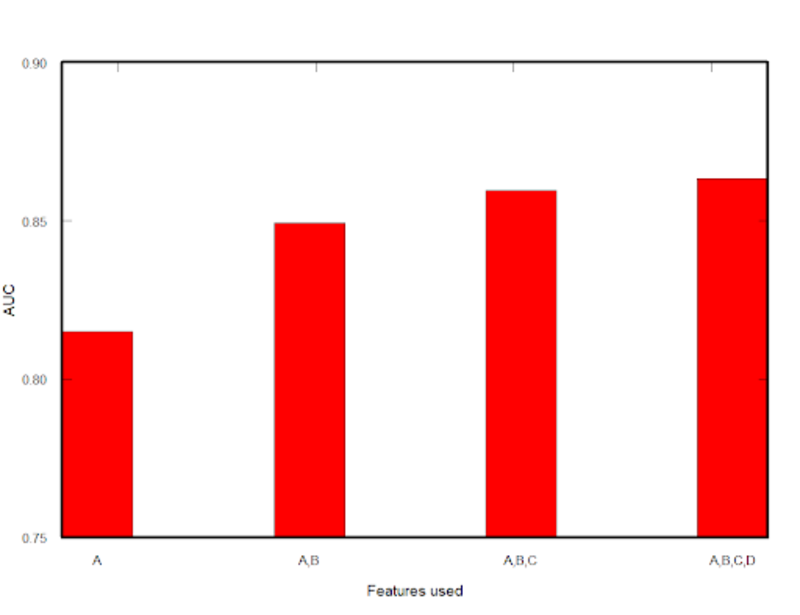
\includegraphics[width=0.7\columnwidth]{img/Fig10_right.pdf}
    \caption{Each curve shows how, given the reputation of the second answerer on a two-answer question, the likelihood of answering second deviates from a uniform baseline as a function of the reputation of the first answerer. The curves on the left (showing the bottom three reputation levels) slope downward, indicating lower reputation levels are more likely to answer questions second if the first answerer also has low reputation; and the curves on the right (showing the top three reputation levels) slope upward, illustrating an analogous homophily by reputation effect}
    \label{fig:fig10}
\end{figure}



\begin{table}[]
	\centering
	\small
	\caption{Important features for predicting task 2}
	\label{tab:18features}
	\resizebox{\columnwidth}{!}{%
\begin{tabular}{|l|l|}
\hline
Sa` & \begin{tabular}[c]{@{}l@{}}questioner reputation, \#of questioner’s questions, and \# of \\ questioner’s answers\end{tabular}                                                                                                                                                     \\ \hline
Sb` & \begin{tabular}[c]{@{}l@{}}\# favorites on question, maximum answer score, maximum\\ answerer reputation, and positive and negative question votes\end{tabular}                                                                                                                   \\ \hline
Sc` & \begin{tabular}[c]{@{}l@{}}average answerer reputation, \# positive votes on last answer,\\ \# negative votes on 2nd answer, length of highest-scoring answer,\\ length of answer given by highest-reputation answerer, \\ and \# comments on highest-scoring answer\end{tabular} \\ \hline
Sd` & \begin{tabular}[c]{@{}l@{}}average time difference between answers, time difference between\\ last 2 answers, time-rank of highest-scoring answer, and time-rank\\  of answer, by highest-reputation answerer.\end{tabular}                                                       \\ \hline
\end{tabular}}
\end{table}



\textbf{Experimentation Results}
With different values of ‘k’, we show the results in table. It is also interesting to observe that as the value of k goes high, users rich in reputation provide bounties others’ questions. The result is shown in Table~\ref{tab:kvalues}.

Due to the absence of a baseline (as present in prediction task 1), we take agglomerative addition of features Sb`, Sc` and Sd` in a baseline Sa` feature set to compute AUC and Accuracy metrics as shown in Fig~\ref{fig:fig10}.

We found that a core set of 18 features that impact this prediction in Table~\ref{tab:18features}. It is noted that addition of set Sd` in Sa`b`c` increases both Accuracy and AUC by less than 2 units, indicating low impact of time-based features in predicting whether a question has been sufficiently answered. 

